% =============================================================================
% APPENDIX — SWE-Bench-Lite analogue of Section 5 (Behavioural / Failure-mode)
% Behavioural and failure-mode analysis on the SWE-Bench-Lite test split,
% computed from three independent evaluation runs of each checkpoint and
% reported as means over the three runs.
% Move this file into the appendix wherever desired.
% =============================================================================

\section{Behavioural Analysis on SWE-Bench-Lite}
\label{app:behavior_lite}

This appendix replicates Section~\ref{sec:analysis} on the
SWE-Bench-Lite test split ($300$ instances). The same trajectory-parsing
pipeline and failure-mode taxonomy are used; as in the main analysis, every
trajectory-level statistic is computed over \emph{three independent
evaluation runs} of each checkpoint and reported as the run-mean.

The qualitative trends documented on Verified hold on Lite: mid-training
raises the recovery rate from $18.8\%$ to $22.1\%$, eliminates the no-patch
failure mode entirely (baseline averages $\sim\!8$ no-patch failures per run,
ours averages $0$), and increases edit iteration on solved trajectories from
$4.4$ to $7.8$ \texttt{str\_replace} operations per task.
The \emph{multi-function} concentration of gain that we documented on
Verified is not visible on Lite because Lite contains no multi-file tasks
and only $54$ multi-function single-file tasks; the bulk of Lite is
single-function single-file tasks, on which the gain is $+4.9$~pp
($19.5\% \to 24.4\%$).

% -----------------------------------------------------------------------------
% TABLE — trajectory metrics on Lite
% -----------------------------------------------------------------------------
\begin{table}[h]
\centering
\caption{Trajectory-level behavioural metrics on SWE-Bench-Lite (14B,
r2e-gym pipeline), averaged over three independent evaluation runs of each
checkpoint. Definitions match Table~\ref{tab:behavior}.}
\label{tab:behavior_lite}
\small
\setlength{\tabcolsep}{4pt}
\begin{tabular}{l c c c c c c c}
\toprule
& \multicolumn{2}{c}{Steps / task}
& \multicolumn{2}{c}{Edits / task}
& \multicolumn{2}{c}{Errors enc.}
& Recovery \\
\cmidrule(lr){2-3}\cmidrule(lr){4-5}\cmidrule(lr){6-7}
Setting & solved & unsolved & solved & unsolved & solved & unsolved & rate (\%) \\
\midrule
+ r2e-gym
  & 17.5 & 21.3 & 4.4 & 5.2 & 4.8 & 5.4 & 18.8 \\
\textbf{+ FIM-Midtrain + r2e-gym}
  & \textbf{24.6} & \textbf{31.7} & \textbf{7.8} & \textbf{11.1}
  & \textbf{5.7} & \textbf{7.5} & \textbf{22.1} \\
\midrule
\multicolumn{8}{l}{\textit{Output and context summaries}} \\
\midrule
& \multicolumn{2}{c}{Empty patch (\% failed)}
& \multicolumn{2}{c}{Loc.\ correct (\% all)}
& \multicolumn{2}{c}{Ctx @ success (tok)}
& Pass (\%) \\
\cmidrule(lr){2-3}\cmidrule(lr){4-5}\cmidrule(lr){6-7}
+ r2e-gym
  & \multicolumn{2}{c}{$3.3$} & \multicolumn{2}{c}{$65.0$}
  & \multicolumn{2}{c}{$13{,}958$} & 18.0 \\
\textbf{+ FIM-Midtrain + r2e-gym}
  & \multicolumn{2}{c}{$\mathbf{0.0}$} & \multicolumn{2}{c}{$\mathbf{71.0}$}
  & \multicolumn{2}{c}{$\mathbf{18{,}104}$} & \textbf{22.0} \\
\bottomrule
\end{tabular}
\end{table}

Failure-mode counts on Lite move in the same direction as on Verified: the
no-patch mode is eliminated ($\sim\!8 \to 0$ trajectories per run),
localisation errors fall by about $11$, and patch errors rise by about $7$,
reflecting the same iterate-and-verify shift.

% -----------------------------------------------------------------------------
% FIGURE — pass rate by gold-patch shape on Lite
% -----------------------------------------------------------------------------
\begin{figure}[h]
\centering
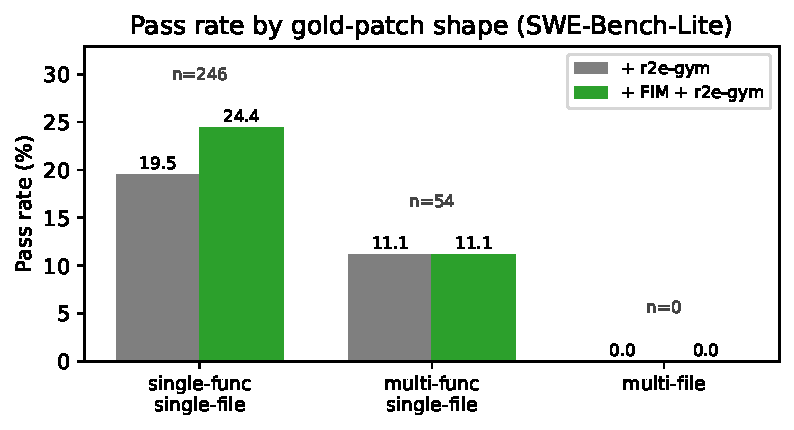
\includegraphics[width=0.62\linewidth]{figs/passrate_by_patchshape_lite.pdf}
\caption{Pass rate on SWE-Bench-Lite stratified by gold-patch shape,
averaged over three evaluation runs per checkpoint. Lite contains no
multi-file tasks; the multi-function single-file bucket is small ($n{=}54$)
and shows no gain on this slice, with the $+4.0$~pp end-task improvement
coming entirely from the single-function single-file bucket ($n{=}246$,
$+4.9$~pp).}
\label{fig:failure_lite}
\end{figure}

\paragraph{Per-instance head-to-head.}
Aggregating per-task outcomes across the three runs (run-majority vote per
checkpoint), the differential favours ours on Lite by a $\sim\!1.8\times$
ratio overall and by a $\sim\!2.1\times$ ratio on the single-function
single-file bucket. On the multi-function single-file bucket the
differential is balanced, consistent with the small absolute number of
such tasks in Lite.
